\documentclass[10pt]{article}

\usepackage[margin=0.75in]{geometry}
\usepackage{amsmath, amssymb}
\usepackage{graphicx}
\usepackage{float}
\usepackage{booktabs}
\usepackage{hyperref}
\usepackage{caption}

\title{\textbf{Comparing Numerical Solvers and Physics-Informed Neural Networks for the Damped Harmonic Oscillator}}
\author{Yiming Ma}
\date{March 16 2026}

\begin{document}

\maketitle

\section*{Introduction}
The damped harmonic oscillator is a classical dynamical system that appears in many physical and engineering applications, including mechanical vibration, structural dynamics, and electrical circuits. Its behavior is governed by the second-order ordinary differential equation
\[
m\ddot{x} + c\dot{x} + kx = 0,
\]
where $m$ is the mass, $c$ is the damping coefficient, and $k$ is the spring constant. Because the damping term dissipates energy, the oscillation amplitude decreases over time.

This project compares three approaches for solving the damped harmonic oscillator: the explicit Euler method, the fourth-order Runge--Kutta (RK4) method, and a simple Physics-Informed Neural Network (PINN). The goal is to evaluate their accuracy and discuss the advantages and limitations of classical numerical solvers versus scientific machine learning methods.

\section*{Method}
In this project, the parameters were chosen as
\[
m = 1.0, \quad c = 0.4, \quad k = 4.0,
\]
with initial conditions
\[
x(0) = 1.0, \quad \dot{x}(0) = 0.0.
\]
The time interval was set to $t \in [0,10]$.

To solve the problem numerically, the second-order equation was rewritten as a first-order system:
\[
x' = v,
\]
\[
v' = -\frac{c}{m}v - \frac{k}{m}x.
\]

A reference solution was first generated using \texttt{solve\_ivp} from SciPy. This reference was used to evaluate the accuracy of the other methods.

Two classical numerical solvers were implemented: the explicit Euler method and RK4. Their predicted displacement curves were compared against the reference solution, and their mean squared errors (MSE) were computed.

A simple PINN was then constructed using a fully connected neural network with two hidden layers and \texttt{tanh} activation functions. Instead of relying on labeled training data, the PINN was trained by minimizing a loss function that included both the differential equation residual and the initial condition constraints:
\[
\mathcal{L} = \mathcal{L}_{\text{physics}} + \mathcal{L}_{\text{IC}}.
\]
This allowed the network to learn a function $x(t)$ that approximately satisfies the governing equation and initial conditions.

\section*{Results}
Figure~\ref{fig:reference} shows the reference solution of the damped harmonic oscillator. The displacement exhibits underdamped oscillatory behavior with gradually decaying amplitude.

\begin{figure}[H]
    \centering
    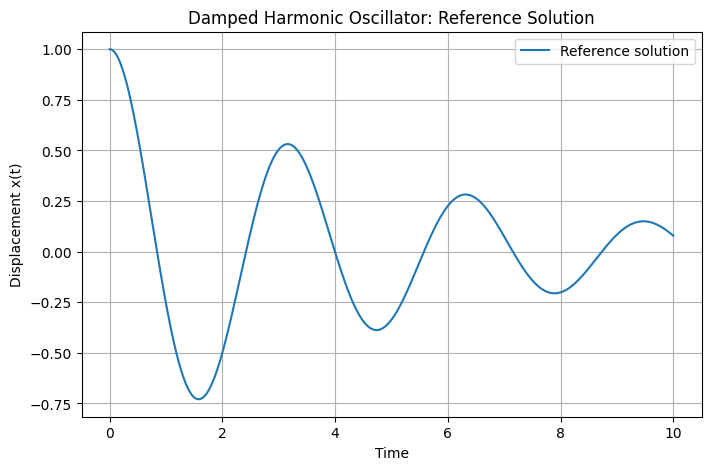
\includegraphics[width=0.75\linewidth]{../figures/reference_solution.png}
    \caption{Reference solution of the damped harmonic oscillator.}
    \label{fig:reference}
\end{figure}

Figure~\ref{fig:euler_rk4} compares the Euler and RK4 solutions with the reference solution. Both methods capture the general oscillatory behavior, but RK4 tracks the reference much more closely than Euler.

\begin{figure}[H]
    \centering
    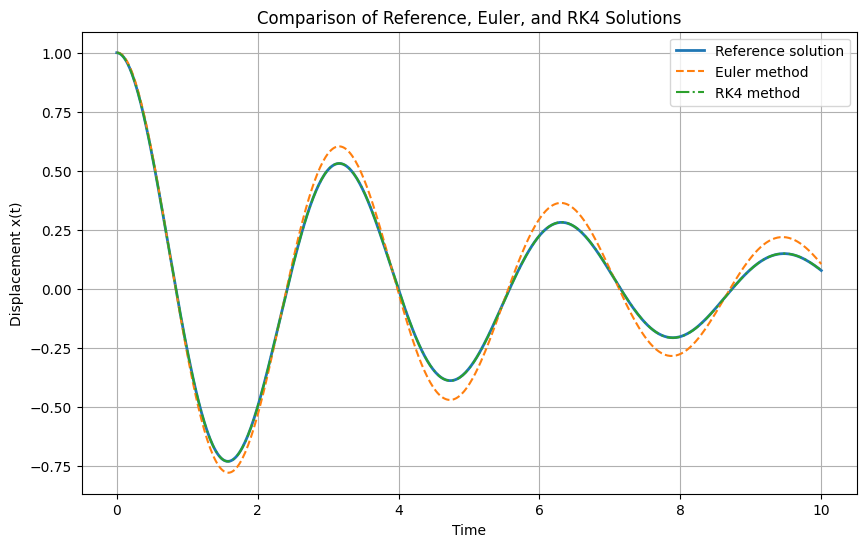
\includegraphics[width=0.75\linewidth]{../figures/euler_rk4_comparison.png}
    \caption{Comparison of the reference, Euler, and RK4 solutions.}
    \label{fig:euler_rk4}
\end{figure}

The error comparison in Figure~\ref{fig:euler_rk4_error} shows that RK4 maintains a much smaller absolute error over time.

\begin{figure}[H]
    \centering
    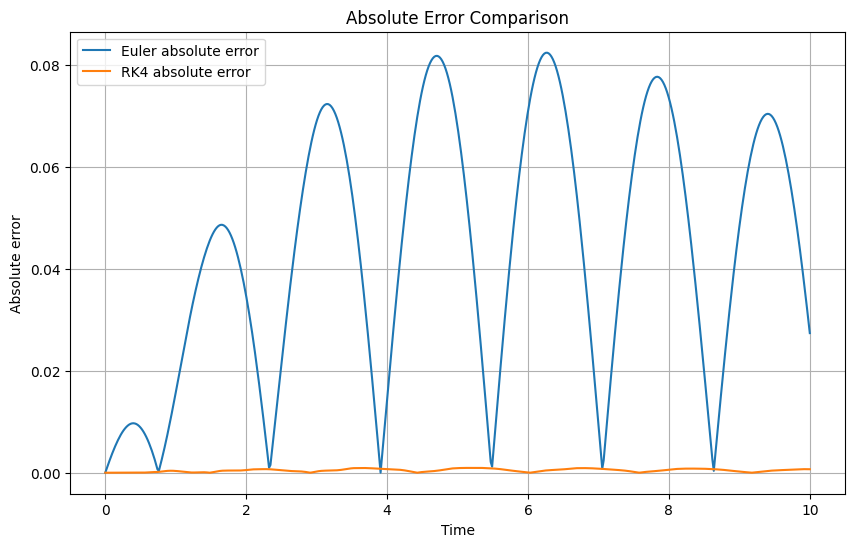
\includegraphics[width=0.75\linewidth]{../figures/euler_rk4_error.png}
    \caption{Absolute error comparison for Euler and RK4.}
    \label{fig:euler_rk4_error}
\end{figure}

The numerical MSE values were:
\[
\text{Euler MSE} \approx 2.51 \times 10^{-3},
\]
\[
\text{RK4 MSE} \approx 3.04 \times 10^{-7}.
\]
These results confirm that RK4 is significantly more accurate than Euler for this problem.

For the PINN, the training loss decreased steadily during optimization, indicating that the model was learning to satisfy both the governing equation and the initial conditions. However, the final PINN prediction deviated noticeably from the reference solution, especially at later times. The PINN MSE was
\[
\text{PINN MSE} \approx 2.06 \times 10^{-2},
\]
which was larger than both Euler and RK4 in this experiment.

\begin{figure}[H]
    \centering
    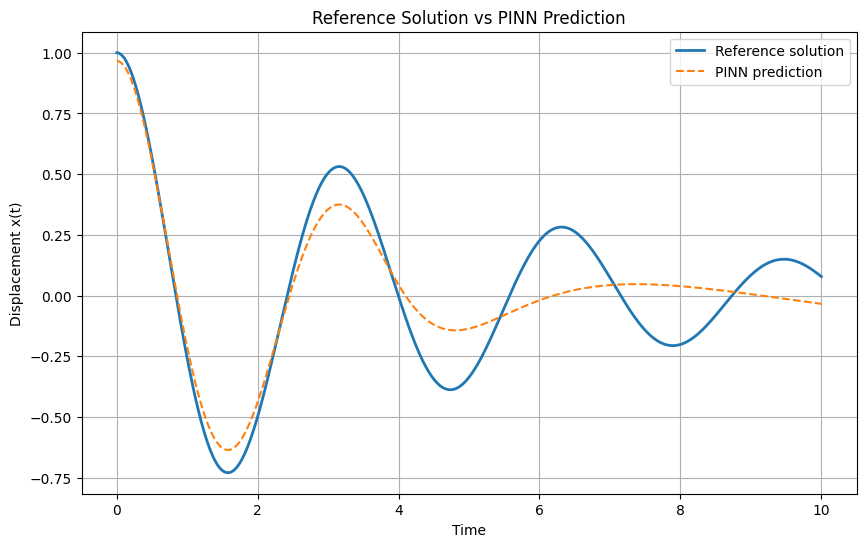
\includegraphics[width=0.75\linewidth]{../figures/pinn_vs_reference.png}
    \caption{Comparison of the reference solution and PINN prediction.}
    \label{fig:pinn_vs_reference}
\end{figure}

\section*{Discussion}
Among the three tested methods, RK4 produced the most accurate solution by a large margin. Euler was able to approximate the overall dynamics, but accumulated larger numerical errors over time. The basic PINN captured the qualitative damped oscillatory trend, but its quantitative accuracy was limited.

This result is reasonable because RK4 is a high-order numerical solver specifically designed for ordinary differential equations, while the PINN must learn the solution indirectly through optimization. For a simple low-dimensional ODE such as the damped harmonic oscillator, classical numerical solvers remain more efficient and reliable. Nevertheless, PINNs are still important because they can incorporate physical laws directly into the learning process and may be more useful for problems where data are sparse, equations are partially known, or traditional solvers become difficult to apply.

\section*{Conclusion}
This project compared Euler, RK4, and a simple PINN for solving the damped harmonic oscillator. RK4 achieved the highest accuracy, Euler gave moderate accuracy, and the PINN successfully learned the qualitative behavior but with the largest error. These results show that classical numerical methods are still highly effective for simple ODEs, while PINNs provide a flexible scientific machine learning framework that may become more competitive with additional tuning or in more complex settings.

\end{document}
